\subsection{Slučaj upotrebe: Kreiranje filmskog projekta}

\subsubsection*{Kratak opis}

Producent kreira novi projekat animiranog filma unosom osnovnih podataka.
Sistem projektu dodeljuje jedinstvenu šifru i status ,,U pripremi'', čime
projekat postaje dostupan za formiranje produkcionog tima i planiranje budžeta
i rokova.

\subsubsection*{Akteri}
\begin{itemize}
    \item \textbf{Producent} -- kreira projekat i odgovoran je za njega.
\end{itemize}

\subsubsection*{Preduslovi}
\begin{itemize}
    \item Producent je prijavljen na sistem.
\end{itemize}

\subsubsection*{Postuslovi}
\begin{itemize}
    \item Projekat je sačuvan u sistemu sa jedinstvenom šifrom i statusom ,,U pripremi''.
    \item Producent je upisan kao odgovorno lice za projekat.
    \item Projekat je dostupan za formiranje produkcionog tima i planiranje budžeta i rokova.
\end{itemize}

\subsubsection*{Osnovni tok}
\begin{enumerate}
    \item Producent bira opciju ,,Kreiraj projekat''.
    \item Sistem prikazuje formu za unos osnovnih podataka o projektu.
    \item Producent popunjava formu i potvrđuje unos.
    \item Sistem proverava ispravnost podataka i da li projekat sa istim nazivom već postoji.
    \item Sistem čuva projekat sa statusom ,,U pripremi'', dodeljuje mu jedinstvenu šifru i upisuje producenta kao odgovorno lice.
    \item Sistem prikazuje stranicu novog projekta sa opcijama za formiranje produkcionog tima i planiranje budžeta i rokova.
\end{enumerate}

\subsubsection*{Podtokovi: /}

\subsubsection*{Alternativni tokovi}

\paragraph*{A1: Nepopunjena ili neispravna polja}
\begin{itemize}
    \item Ovaj tok se dešava u koraku 4 osnovnog toka, ako neko obavezno polje nije popunjeno ili je neispravno (npr. ciljno trajanje nije pozitivan broj).
    \item Sistem označava polja koja treba ispraviti i prikazuje poruku o grešci.
    \item Producent ispravlja podatke.
    \item Povratak na korak 3 osnovnog toka.
\end{itemize}

\paragraph*{A2: Projekat sa istim nazivom već postoji}
\begin{itemize}
    \item Ovaj tok se dešava u koraku 4 osnovnog toka, ako u sistemu već postoji projekat sa istim nazivom.
    \item Sistem obaveštava producenta da naziv već postoji.
    \item Producent unosi drugi naziv.
    \item Povratak na korak 3 osnovnog toka.
\end{itemize}

\subsubsection*{Specijalni zahtevi}
\begin{itemize}
    \item Šifra projekta je jedinstvena i ne menja se nakon dodele.
    \item Sistem beleži ko je i kada kreirao projekat.
\end{itemize}

\subsubsection*{Dodatne informacije}
\begin{itemize}
    \item Osnovni podaci o projektu (koraci 2 i 3): naziv filma, žanr, kratak opis (sinopsis), ciljno trajanje filma i naručilac.
    \item Status projekta: ,,U pripremi'' (posle kreiranja).
    \item Produkcioni tim se formira u slučaju upotrebe ,,Formiranje produkcionog tima'', a budžet i rokovi se planiraju u slučaju upotrebe ,,Upravljanje budžetom i rokovima''.
\end{itemize}


\begin{figure}[H]
	\centering
	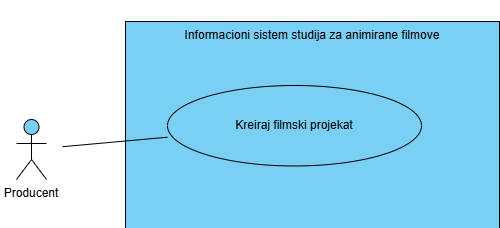
\includegraphics[width=\textwidth]{./dijagrami/dijagrami_slucajeva_upotrebe/kreiranje_filmskog_projekta.png}
	\caption{Dijagram slučaja upotrebe ,,Kreiranje filmskog projekta''}
 \end{figure}

\begin{figure}[H]
	\centering
	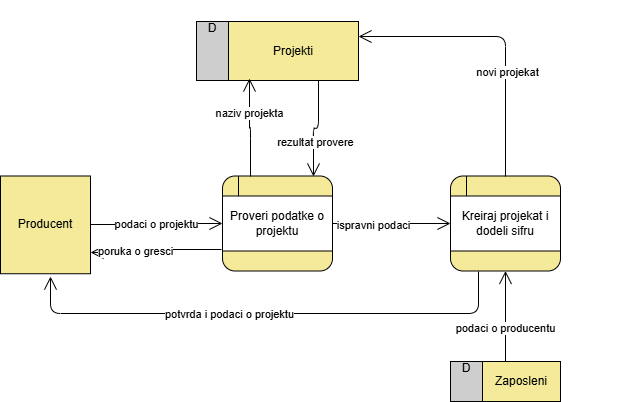
\includegraphics[width=\textwidth]{./dijagrami/dfd/kreiranje_filmskog_projekta.png}
	\caption{Dijagram toka podataka ,,Kreiranje filmskog projekta''}
 \end{figure}

\newpage
